\documentclass{article}
\usepackage[spanish]{babel}
\usepackage{amsmath}
\usepackage[right=2cm,left=3cm,top=2cm,headsep=0.5cm,footskip=0.5cm]{geometry}
\usepackage{graphicx}
\usepackage{latexsym}
\usepackage{eufrak}
\usepackage{dsfont}
\usepackage{hyperref}
\usepackage{enumerate} 
\usepackage{lscape}
\usepackage{natbib}
\usepackage{booktabs}
\usepackage{adjustbox}


\usepackage{titlesec}
\usepackage{fancyhdr}

\usepackage[utf8]{inputenc}
\usepackage[T1]{fontenc}
\usepackage{times}

\usepackage{color}
\definecolor{gray97}{gray}{.97}
\definecolor{gray75}{gray}{.75}
\definecolor{gray45}{gray}{.45}

\usepackage{listings}
\lstset{ frame=Ltb,
framerule=0pt,
aboveskip=0.5cm,
framextopmargin=3pt,
framexbottommargin=3pt,
framexleftmargin=0.4cm,
framesep=0pt,
rulesep=.4pt,
backgroundcolor=\color{gray97},
rulesepcolor=\color{black},
%
stringstyle=\ttfamily,
showstringspaces = false,
basicstyle=\small\ttfamily,
commentstyle=\color{gray45},
keywordstyle=\bfseries,
%
numbers=left,
numbersep=15pt,
numberstyle=\tiny,
numberfirstline = false,
breaklines=true,
}

% minimizar fragmentado de listados
\lstnewenvironment{listing}[1][]
{\lstset{#1}\pagebreak[0]}{\pagebreak[0]}

\lstdefinestyle{consola}
{basicstyle=\scriptsize\bf\ttfamily,
backgroundcolor=\color{gray75},
}

\lstdefinestyle{Python}
{language=Python,
}

\title{Pr\'actica CMB}

\newtheorem{teo}{\underline{Teorema}}
\newtheorem{defi}{\underline{Definici\'on}}
\newtheorem{propo}{\underline{Proposici\'on}}
\newtheorem{ejem}{\underline{Ejemplo}}[section]
\newtheorem{prob}{\underline{Problema}}
\newtheorem{lema}{\underline{Lema}}
\newtheorem{obs}{\underline{Observaci\'on}}[section]




\title{Fuentes de rayos $\gamma$: IC 310}
\author{Jannis Necker$^{1}$, Santiago Arranz$^{1}$ \\ \\
\small{$^{1}$Universidad Complutense de Madrid}}

\begin{document}
\subsubsection*{Santiago Arranz Sanz}
\subsubsection*{FÍSICA DEL MODELO COSMOLÓGICO ESTÁNDAR}

\section*{Estudio de la dependencia del espectro angular de temperatura del CMB con los parámetros cosmológicos.}

El \textbf{objetivo} de la práctica es estudiar la dependencia del espectro angular de fluctuaciones de temperatura $C_l$ con los parámetros:
\begin{enumerate}
\item \textbf{$h$}: El parámetro de Hubble normalizado.
\item \textbf{$\omega_b$}: El parámetro de densidad bariónica.
\item \textbf{$n_s$}: Parámetro que define la potencia de la función del espectro de potencias:
$$P_R(k)=A_s\left(\frac{k}{k_0}\right)^{n_s-1}$$
donde $A_s=2.20\times 10^{-9}$ y $k_0=0.05$ Mpc$^{-1}$.
\end{enumerate}

\begin{figure}[h]
\centering
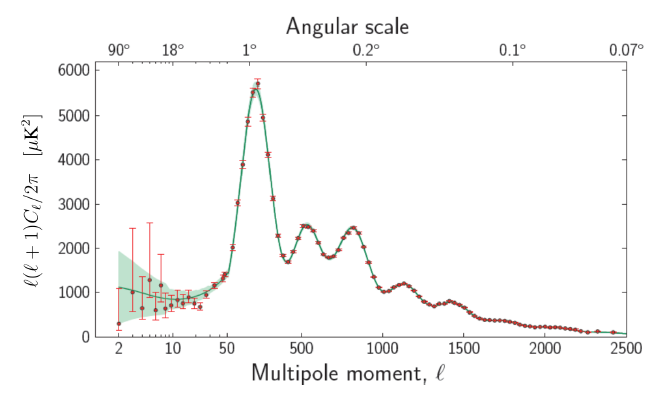
\includegraphics[scale=0.8]{Captura.PNG}
\end{figure}

Para ello vamos a usar los siguietes paquetes de \textit{Python} y todas las funciones que definamos las haremos depender de estos parámetros.
\begin{lstlisting}[style=Python]
import numpy as np
import pandas as pd
import scipy as sp
import scipy.integrate as integrate
import matplotlib.pyplot as plt
\end{lstlisting}

\subsection*{Parámetros y funciones a usar.}
En el guión de la práctica hemos recibido un listado y guía para construir una aproximación a la función $C_l$ solamente valida para $l>>100$, el cual solo tiene en cuenta el efecto *Sachs-Wolfe* ignorando las contribuciones Doppler y el efecto *Sachs-Wolfe integrado*.
$$C_l(z)\simeq 4\pi\frac{9}{25}\int P_R(k)\left[-R(z_{dec})T(k/k_{eq})+\frac{5}{3}\cos(k\cdot r_s)e^{-k^2/k_D^2}\right]^2\ j_l^2(k(\eta_0-\eta_{dec}))\frac{dk}{k}$$

Las funciones y parámetros que forman parte de dicha aproximación pasarán a ser definidas a continuación. Primero definimos la constante de Hubble normalizada $h=0.67\ \text{km}/\text{s}^{-1}$ y su versión sin normalizar $H_0=h/2998\ \text{Mpc}^{-1}$. Los parámetros que indican la densidad de energía de bariones $\omega_b$, de radiación $\omega_r$, materia $\omega_m$ y de energía del vacío $\omega_\Lambda$ están definidos como:
$$\omega_m=0.14\quad ;\quad \omega_b=0.022\quad ; \quad \omega_r=\left(1+\frac{7}{8}N_{eff}\left(\frac{4}{11}\right)^{4/3}\right)\omega_\gamma= 4.17\times 10^{-5}$$
donde $N_{eff}$ es el número efectivos de neutrinos y $\omega_\gamma$ la denisdad de energía de neutrinos. Además $\omega_\lambda$ la podmeos definir como una función de $h$:
$$\omega_\lambda(h)=h^2-\omega_m-\omega_r$$
\begin{lstlisting}[style=Python]
h=0.67
w_b=0.022
w_m=0.14
w_r=4.17*10**(-5)
w_lamb=lambda t: t**2-w_m-w_r
H=lambda t: t/2998
H_0=H(h)
\end{lstlisting}

Podemos definir la velocidad del sonido en función del redshift $z$ y de la densidad de energía de materia barionica $\omega_b$ como:
$$
c_s^2=\frac{1}{3}\frac{1}{1+R(z,\omega_b)}\quad \text{donde}\quad R(z,\omega_b)=\frac{3.04\times 10^{4}}{1+z}\omega_b
$$
Para hemos usado las funciones lambdas y hemos marcado por defecto de $\omega_b$ el estipulado más arriba.

\begin{lstlisting}[style=Python]
R=lambda z,wb=w_b:wb*(3.04*10**4)/(1+z)
c_s=lambda z,wb=w_b:np.sqrt( (1/3)/(1+R(z, wb)) )
\end{lstlisting}

Para definir el horizonte del sonido en el momento del desacople $z_{dec}=1090.3$ usamos la aproximación a un universo plano, la definición de la ecuación del movimiento usando que $\omega_\alpha=h^2\Omega_\alpha$ con $\alpha=r,m,\Lambda$:
$$
H(z)^2=H_0^2\frac{\left[(1+z)^3\omega_m+(1+z)^4\omega_r+\omega_\Lambda\right]}{h^2}=H_0^2\cdot E(z)^2
$$
Para definir el radio del horizonte de sonido trabajamos con coordenadas de comovimiento sabiendo que $dr/dt=a\cdot dx/dt=c_s(t)$, donde $a(t)$ es el factor de escala. Usando que $dt=da/(a\cdot H(a))=da/(a\cdot H_0E(a))$ obtenemos si integramos y usamos que $a=(1+z)^{-1}$

$$
r_s=\int_0^{a_{dec}}\frac{c_s(a)}{a^2H_0E(a)}da=H_0^{-1}\int_{z_{dec}}^\infty\frac{c_s(z)}{E(z)}dz 
$$

\begin{lstlisting}[style=Python]
z_dec=1090.3
def E(z,hf=h):
    wl=w_lamb(hf)
    parte1=w_m*np.power((1+z),3) + w_r*np.power((1+z),4) + wl
    return (np.sqrt(parte1)/hf)

r_s=lambda h_p=h,wb=w_b: integrate.quad(lambda z: c_s(z,wb)/E(z,hf=h_p),z_dec,np.inf)[0]/H(h_p)
\end{lstlisting}

Para definir el tiempo conforme desde el desacoplo $\eta_0-\eta_{dec}$ usamos un desarrollo parecido al anterior:
$$
d_A^c(z_{dec})=\eta_0-\eta_{dec}=\int_{t_0}^{t_{dec}} \frac{dt}{a}=\int_{a_0}^{a_{dec}} \frac{da}{a^2H}=H_0^{-1}\int_0^{z_dec} \frac{1}{E(z)}dz
$$

\begin{lstlisting}[style=Python]
d_A = lambda h_p=h: integrate.quad(lambda z: 1/E(z,h_p),0,z_dec)[0]/H(h)
\end{lstlisting}

Definimos la función de transferencia:
$$T(x)=\frac{\ln(1+0.171x)}{0.171x}\left[1 + 0.284x + 1.18x^2 + 0.399x^3 + 0.49x^4\right]^{-0.25}$$
y las escalas deigualdad $k_{eq}=0.073\omega_m$ Mpc$^{-1}$ y de Silk $k_D\simeq 0.14$ Mpc$^{-1}$. Recordar que la relación entre escala y multipolos viene dada por $l\simeq k d_A^c(z_{dec})$.
\begin{lstlisting}[style=Python]
def T(x):
    parte1=np.log(1+0.171*x)/(0.171*x)
    parte2=(1 + 0.284*x + np.power(1.18*x,2) + np.power(0.399*x,3) + np.power(0.49*x,4))**(-0.25)
    return parte1*parte2
k_eq=0.073*w_m
k_d=0.14
\end{lstlisting}

Por último definimos la función del espectro de potencias con sus parámetros $A_s=2.20\times 10^{-9}$, $k_0=0.05$ Mpc$^{-1}$ y $n_s=0.97$.

$$P_R(k)=A_s\left(\frac{k}{k_0}\right)^{n_s-1}$$

y la función de Bessel esférica para $l$ usando la aproximación:
$$
j_l^2(x)=\begin{cases}
\left[4x^2(x^2-l^2)\right]^{-1/2} & x>l\\
0 & x<l
\end{cases}
$$

\begin{lstlisting}[style=Python]
ns=0.97
A_s=2.2*10**(-9)
k_0=0.05
P_R=lambda k,n=ns: A_s*((k/k_0)**(n-1))
def func_bessel(x,l):
    if x>l:
        return 0.5/(x*np.sqrt(np.power(x,2)-np.power(l,2)))
    else:
        return 0
\end{lstlisting}

\subsection*{Función del espectro angular de temperaturas del CMB}
Una vez definido todas las partes de $C_l$ pasemos a definirla también a esta:
$$C_l(z)\simeq 4\pi\frac{9}{25}\int P_R(k)\left[-R(z_{dec})T(k/k_{eq})+\frac{5}{3}\cos(k\cdot r_s)e^{-k^2/k_D^2}\right]^2\ j_l^2(k(\eta_0-\eta_{dec}))\frac{dk}{k}$$

\begin{lstlisting}[style=Python]
def c_l_funcion(l,Rz=R(z_dec),dA=d_A(),rs=r_s(),n_s=ns):
    def func_int(k):
        const=4*np.pi*9/25
        parte1=P_R(k,n_s)
        parte2=np.power(-Rz*T(k/k_eq)+5/3*np.cos(k*rs)*np.exp(-(k/k_d)**2),2)
        parte3=func_bessel(k*dA,l)/k
        return parte1*parte2*parte3

    limite_sup=4000/(dA)
    limite_inf=l/(dA)
    resultado=integrate.quad(func_int,limite_inf,limite_sup)[0]
    constante=4*np.pi*9/25
    return resultado*constante
\end{lstlisting}

Definido todas las funciones y descrito el comportamiento de las anisotropías de temperatura del CMB pasemos a resolver los ejercicios planteados en la práctica.

\section{Ejercicio 1}

\begin{quote}
\textit{Fijando los valores de los parámetros a los de la cosmología estándar: $h = 0.67;\quad \omega_b = 0.022;\quad \omega_m = 0.14;\quad n_s = 0.97$:*
\begin{enumerate}
\item Calcular $R(z_{dec})$, $r_s$ y $d_A^c(z_{dec})$. 
\item Representar gráficamente $l(l+1)c_l/(2\pi)$ para $l\in[100,1500]$.
\end{enumerate}
}
\end{quote}

\subsection{ Sacar los valores de $R(z_{dec}), d_A^c$ y $r_s$}
Obtenemos los valores de la \textbf{Tabla \ref{tab:1}}
\begin{lstlisting}[style=Python]
dic={'$R(z_{dec})$':[R(z_dec)],"$d_A^c(z_{dec})$":[d_A()],"$r_s$":[r_s()]}
tabla=pd.DataFrame(dic)
tabla
\end{lstlisting}

\begin{table}[h]
\centering
\begin{tabular}{rrr}
\toprule
  $R(z_{dec})$ &  $d_A^c(z_{dec})$ & $r_s$ \\
\midrule
      0.612847 &       14002.47092 &  145.327004 \\
\bottomrule
\end{tabular}
\caption{\label{tab:1} Valores de $R(z_{dec}), d_A^c(z_{dec})$ y $r_s$}
\end{table}

\subsection{Representar gráficamente el espectro angular de temperaturas del CMB}
Vamos a recorres los valores del intervalo $[100,1500]$ y guardaremos los $C_l$ en un vector para posteriormente representarlos gráficamente en la \textbf{Figura \ref{fig:1}}.
\begin{lstlisting}[style=Python]
l_minimo=100
l_maximo=2500
l_array=np.array(range(l_minimo,l_maximo))
longitud=len(l_array)
cl=np.zeros(longitud)
i=0    
for l in l_array:
    valor=c_l_funcion(l,R(z_dec))
    cl[i]=valor*l*(l+1)/(2*np.pi)
    i+=1

plt.figure(figsize=(10,7))
plt.title("Espectro Angular de Temperaturas", fontsize=20)
plt.ylabel("$l(l+1)C_l/2\pi\ [\mu K^2]$", fontsize=16)
plt.xlabel("Multipole moment, $l$", fontsize=16)
plt.plot(l_array,cl*10**12)
plt.savefig("Espec.png")
plt.show()     
plt.close()
\end{lstlisting}

\begin{figure}[h]
    \begin{center}
    \adjustimage{max size={0.9\linewidth}{0.9\paperheight}}{output_30_0.png}
    \end{center}
    \caption{\label{fig:1} Espectro angular de Temperaturas del CMB.}
\end{figure}

\section{Ejercicio 2}
\begin{quote}
\textit{Estudiar la dependencia del espectro en los parámetros  $R(z_{dec})$, $r_s$ y $d_A^c(z_{dec})$ variando cada uno de ellos independientemente.}
\end{quote}

Vamos a definir cuatro tipos de coeficientes de variación $\sigma=0.5,1,1.5,2$ y veremos cuales son los efectos de las variaciones de  $R(z_{dec})\cdot\sigma$, $r_s\cdot\sigma$ y $d_A^c(z_{dec})\cdot\sigma$ en el $C_l$. Primero empezaremos por $R(z_{dec})$ en la figura \ref{fig:2}.
\begin{lstlisting}[style=Python]
variacion=np.array([1,0.5,1.5,2])
paso=len(variacion)

plt.figure(figsize=(10,7))
dA=d_A()
rs=r_s()
for j in range(0,paso):
    sig=variacion[j]
    l_minimo=100
    l_maximo=1501
    l_array=np.array(range(l_minimo,l_maximo))
    longitud=len(l_array)
    cl=np.zeros(longitud)
    i=0    
    for l in l_array:
        valor=c_l_funcion(l,R(z_dec)*sig,dA,rs)
        cl[i]=valor*l*(l+1)/(2*np.pi)
        i+=1
    
    plt.plot(l_array,cl*10**12,label="$R_z=R(z_d)*{:.2f}$".format(sig))

plt.title("Espectro Angular de Temperaturas, Variacion en $R(z_{dec})$", fontsize=20)
plt.ylabel("$l(l+1)C_l/2\pi\ [\mu K^2]$", fontsize=16)
plt.xlabel("Multipole moment, $l$", fontsize=16)
plt.legend()
plt.savefig("Espec_R_z.png")
plt.show()
plt.close()
\end{lstlisting}

\begin{figure}[h]
    \begin{center}
    \adjustimage{max size={0.9\linewidth}{0.9\paperheight}}{output_33_0.png}
    \end{center}
\caption{\label{fig:2} Espectro angular de Temperaturas del CMB variandp $R(z_{dec})$.}
\end{figure}

Observamos que los picos no se mueven de lugar, sino que solo suben y bajan en su magnitud. Es de resaltar que en los picos pares la proporcionalidad entre el valor de $R(z_{dec})$ y la magnitud de los picos es inversa, es decir, cuanto menor es el valor de $R(z_{dec})$ mayor es la magnitud del pico, mientras que para los picos impares ocurre el efecto contrario.


Calculamos las variaciones para $d_A$ en la \textbf{Figura \ref{fig:3}}.
\begin{lstlisting}[style=Python]
variacion=np.array([1,0.5,1.5,2])
paso=len(variacion)
plt.figure(figsize=(10,7))
Rz=R(z_dec)
rs=r_s()
for j in range(0,paso):
    sig=variacion[j]
    l_minimo=100
    l_maximo=1501
    l_array=np.array(range(l_minimo,l_maximo))
    longitud=len(l_array)
    cl=np.zeros(longitud)
    i=0    
    for l in l_array:
        valor=c_l_funcion(l,Rz,dA=d_A()*sig,rs=rs)
        cl[i]=valor*l*(l+1)/(2*np.pi)
        i+=1
    
    plt.plot(l_array,cl*10**12,label="$d=d_A^c(z)*{:.2f}$".format(sig))

plt.title("Espectro Angular de Temperaturas, Variacion en $d_A^c(z_{dec})$", fontsize=20)
plt.ylabel("$l(l+1)C_l/2\pi\ [\mu K^2]$", fontsize=16)
plt.xlabel("Multipole moment, $l$", fontsize=16)
plt.legend()
plt.savefig("Espec_d_a.png")
plt.show()
plt.close()
\end{lstlisting}

\begin{figure}[h]
    \begin{center}
    \adjustimage{max size={0.9\linewidth}{0.9\paperheight}}{output_35_0.png}
    \end{center}
\caption{\label{fig:3} Espectro angular de Temperaturas del CMB variando $d_A^c(z_{dec})$.}
\end{figure}

Para este caso observamos que los picos se desplazan de izquierda a derecha en función de si son más pequeños o más grandes respectvamente. Con respecto a la magnitud de los picos se observa un ligero crecimiento de magnitud según aumenta el valor de $d_A^c(z_{dec})$.\\

Calculamos las variaciones para $r_s$ en la \textbf{Figura \ref{fig:4}}.
\begin{lstlisting}[style=Python]
variacion=np.array([1,0.5,1.5,2])
paso=len(variacion)
plt.figure(figsize=(10,7))
Rz=R(z_dec)
dA=d_A()
for j in range(0,paso):
    sig=variacion[j]
    l_minimo=100
    l_maximo=1501
    l_array=np.array(range(l_minimo,l_maximo))
    longitud=len(l_array)
    cl=np.zeros(longitud)
    i=0    
    for l in l_array:
        valor=c_l_funcion(l,Rz,dA,rs=r_s()*sig)
        cl[i]=valor*l*(l+1)/(2*np.pi)
        i+=1
    
    plt.plot(l_array,cl*10**12,label="$r=r_s*{:.2f}$".format(sig))

plt.title("Espectro Angular de Temperaturas, Variacion en $r_s$", fontsize=20)
plt.ylabel("$l(l+1)C_l/2\pi\ [\mu K^2]$", fontsize=16)
plt.xlabel("Multipole moment, $l$", fontsize=16)
plt.legend()
plt.savefig("Espec_r_s.png")
plt.show()
plt.close()
\end{lstlisting}

\begin{figure}[h]
    \begin{center}
    \adjustimage{max size={0.9\linewidth}{0.9\paperheight}}{output_37_0.png}
    \end{center}
\caption{\label{fig:4} Espectro angular de Temperaturas del CMB variando $r_s$.}
\end{figure}

Para las variaciones del horizonte del sonido se ve que existe un desplazamiento de izquierda a derecha según el valor de $r_s$ crece o decrece respectivamente y un aumento en la magnitud de los picos con respecto al crecimiento del valor $r_s$.

\section{Ejercicio 3}
\begin{quote}
\textit{Estudiar la dependencia del espectro con $h$. Considerar, aparte del valor estándar, $h = 0.5$ y $h = 0.8$ con el resto de parámetros fijos. Comprobar que el valor de $h$ no afecta a la altura de los picos pero sí a su posición. Explicar este efecto en términos de lo visto en la cuestión 2.}
\end{quote}

De la misma manera que en el ejercicio 2 y dado que hemos definido las funciones que conforman el $C_l$ en función de $h$ vamos a visualizar los cambios de que sufre las anisotropías de temperatura del CMB cuando el valor de $h$ cambia. (\textbf{Figura \ref{fig:5}})

\begin{lstlisting}[style=Python]
paso=3
h_array=np.array([h,0.5,0.8])

plt.figure(figsize=(10,7))
Rz=R(z_dec)
for j in range(0,paso):
    h_l=h_array[j]    
    l_minimo=100
    l_maximo=1501
    l_array=np.array(range(l_minimo,l_maximo))
    longitud=len(l_array)
    cl=np.zeros(longitud)
    i=0    
    
    for l in l_array:
        valor=c_l_funcion(l,Rz,d_A(h_p=h_l),r_s(h_p=h_l))
        cl[i]=valor*l*(l+1)/(2*np.pi)
        i+=1
    
    plt.plot(l_array,cl*10**12,label="$h={:.2f}$".format(h_array[j]))

plt.title("Espectro Angular de Temperaturas, Variacion en $h$", fontsize=20)
plt.ylabel("$l(l+1)C_l/2\pi\ [\mu K^2]$", fontsize=16)
plt.xlabel("Multipole moment, $l$", fontsize=16)
plt.legend()
plt.savefig("Espec_h.png")
plt.show()
plt.close()
\end{lstlisting}

\begin{figure}[h]
    \begin{center}
    \adjustimage{max size={0.9\linewidth}{0.9\paperheight}}{output_42_0.png}
    \end{center}
\caption{\label{fig:5} Espectro angular de Temperaturas del CMB variando $h$}
\end{figure}

Observamos las variaciones muy similares a cuando solo modificabamos $d_A^c(z_{dec})$ en el ejercicio 2. Esto ocurre por la función $E(z)$ definida como:

$$
E(z,h)^2=\frac{(1+z)^3\omega_m+(1+z)^4\omega_r+h^2-\omega_m-\omega_r}{h^2}=\frac{[(1+z)^3-1]\omega_m+[(1+z)^4-1]\omega_r+h^2}{h^2}
$$

sustituyendo en las ecuaciones del horizonte de sonido y del tiempo conforme:
$$
r_s=2998\int_{z_{dec}}^\infty \frac{c_s(z)}{([(1+z)^3-1]\omega_m+[(1+z)^4-1]\omega_r+h^2)^{1/2}}dz
$$

$$
d_A^c(z_{dec})=2998\int_0^{z_{dec}} \frac{dz}{([(1+z)^3-1]\omega_m+[(1+z)^4-1]\omega_r+h^2)^{1/2}}
$$

Vemos que la dependencia en $h$ tanto para el horizonte de sonido como para la distancia del tiempo conforme es la misma sin embargo parece que solo se nota las variaciones en $d_A^c(z_{dec})$. Esto es por los límites de integración de las respectivas integrales. Por un lado tenemos en $d_A^c(z_{dec})$ cuyos límites son entre 0 y 1090, esto hace que las variaciones en $h$ dentro del denominador sean más siginifacitvas que para el horizonte del sonido donde sus límites son 1090 y $\infty$. Esto hace que las variaciones en $r_s$ no seán signifactivas mientras que para $d_A^c(z_{dec})$ sí que lo sean como muestra la siguiente \textbf{Tabla \ref{tab:2}}.

\begin{lstlisting}[style=Python]
R_ar=np.array([R(z_dec)]*3)
d_ar=np.array([d_A(h_p=h),d_A(h_p=0.5),d_A(h_p=0.8)])
r_ar=np.array([r_s(h_p=h),r_s(h_p=0.5),r_s(h_p=0.8)])
dic={'$R(z_{dec})$':R_ar,"$d_A^c(z_{dec})$":d_ar,"$r_s$":r_ar}
tabla=pd.DataFrame(dic)
tabla
\end{lstlisting}

\begin{table}[h]
\centering
\begin{tabular}{rrr}
\toprule
  $R(z_{dec})$ &  $d_A^c(z_{dec})$ & $r_s$ \\
\midrule
      0.612847 &      14002.470920 &  145.327004 \\
      0.612847 &      11022.872357 &  145.327004 \\
      0.612847 &      16134.698481 &  145.327004 \\
\bottomrule
\end{tabular}
\caption{\label{tab:2} Tabla de las variaciones de $h$}
\end{table}

\section{Ejerciio 4}
\begin{quote}
\textit{Estudiar la dependencia del espectro con $\omega_b$. Considerar, aparte del valor estándar, $\omega_b = 0.01$ y $\omega_b = 0.04$ con el resto de parámetros fijos. Comprobar que aumentar $\omega_b$ incrementa los picos impares y disminuye los pares. Explicar este efecto en términos de lo visto en la cuestión 2.}
\end{quote}

De manera similar a antes procedemos a ver las modificaciones que sufre $C_l$ cuando modificamos la cantidad de densidad de energía de bariones. (\textbf{Figura \ref{fig:6}}).
\begin{lstlisting}[style=Python]
w_b1=0.01
w_b2=0.04

paso=3
wb_array=np.array([w_b,w_b1,w_b2])

plt.figure(figsize=(10,7))
dA= d_A()

d_arr=np.array([dA]*3)
R_arr=np.zeros(3)
r_arr=np.zeros(3)
for j in range(0,paso):
    l_minimo=100
    l_maximo=1501
    l_array=np.array(range(l_minimo,l_maximo))
    longitud=len(l_array)
    cl=np.zeros(longitud)
    i=0    
    Rz=R(z_dec,wb=wb_array[j])
    rs=r_s(wb=wb_array[j])
    for l in l_array:
        valor=c_l_funcion(l,Rz,dA,rs)
        cl[i]=valor*l*(l+1)/(2*np.pi)
        i+=1
    R_arr[j]=Rz
    r_arr[j]=rs
    plt.plot(l_array,cl*10**12,label="$\omega_b={:.2f}$".format(wb_array[j]))

plt.title("Espectro Angular de Temperaturas, Variacion en $\omega_b$", fontsize=20)
plt.ylabel("$l(l+1)C_l/2\pi\ [\mu K^2]$", fontsize=16)
plt.xlabel("Multipole moment, $l$", fontsize=16)
plt.legend()
plt.savefig("Espec_wb.png")
plt.show()
plt.close()
\end{lstlisting}

\begin{figure}[h]
    \begin{center}
    \adjustimage{max size={0.9\linewidth}{0.9\paperheight}}{output_48_0.png}
    \end{center}
\caption{\label{fig:6} Espectro angular de Temperaturas del CMB variando $\omega_b$}
\end{figure}

Al igual que ocurría en el ejercicio 2 cuando varíamos el valor de $R(z_{dec})$ los picos de las anisotropías de temperatura del CMB varían en su magnitud, creciendo en el caso de los picos impares y decreciendo en los picos pares. Esto ocurre ya que al variar el valor de $\omega_b$ estamos modificando el valor de $R(z,\omega_b)=\omega_b\cdot 3.04\times 10^4/(1+z)$. Por otro lado vemos una variación en la posición de los picos a diferencia que en el ejercicio 2, esto es porque al variar $\omega_b$ estamos modificando también el valor de $c_s$ del cual depende $r_s$. Estas modificaciones origina una traslación de los picos a la derecha según aumenta $r_s$, al igual que pasaba en el ejercicio 2. Dichas variaciones en estos parametros las podemos observar en la siguiente \textbf{Tabla \ref{tab:3}}

\begin{table}[h]
\centering
\begin{tabular}{rrr}
\toprule
  $R(z_{dec})$ &  $d_A^c(z_{dec})$ & $r_s$ \\
\midrule
      0.612847 &       14002.47092 &  145.327004 \\
      0.278567 &       14002.47092 &  153.797226 \\
      1.114267 &       14002.47092 &  135.476638 \\
\bottomrule
\end{tabular}
\caption{\label{tab:3} Valores de $R(z_{dec}), d_A^c(z_{dec})$ y $r_s$}
\end{table}

\section{Ejercicio 5}
\begin{quote}
\textit{Estudiar la dependencia del espectro con $n_s$. Considerar, aparte del valor estándar, $n_s = 0.7$ y $n_s = 1.2$ con el resto de parámetros fijos. Determinar el multipolo $l$ correspondiente a la escala del pivote $k_0$ y explicar el efecto.}
\end{quote}

Empezaremos igual que en los ejercicios anteriores y marcaremos el multipolo correspondiente a $k_0$ con una línea vertical. Hay que fijarse, dado que $n_s$ solo aparece en $P_R$ dentro de la aproximación de $C_l$, para el multipolo. (\textbf{Figura \ref{fig:7}})

\begin{lstlisting}[style=Python]
paso=3

ns_1=0.7
ns_2=1.2
ns_array=np.array([ns,ns_1,ns_2])

plt.figure(figsize=(10,7))
dA =d_A()
rs=r_s()
Rz=R(z_dec)

l_0=k_0*dA

l_M=0
l_m=50000
for j in range(0,paso):
    l_minimo=100
    l_maximo=1501
    l_array=np.array(range(l_minimo,l_maximo))
    longitud=len(l_array)
    cl=np.zeros(longitud)
    i=0    
    for l in l_array:
        valor=c_l_funcion(l,Rz,dA,rs,ns_array[j])
        constante=4*np.pi*9/25
        cl[i]=valor*l*(l+1)/(2*np.pi)
        i+=1
    
    if np.max(cl*10**12)>l_M : 
        l_M=np.max(cl*10**12)
    if np.min(cl*10**12)<l_m : 
        l_m=np.min(cl*10**12)
        
    plt.plot(l_array,cl*10**12,label="$n_s={:.2f}$".format(ns_array[j]))

vy=np.linspace(l_m,l_M,1000)
vx=np.ones(1000)*l_0
plt.plot(vx,vy,'r:',label="$l_0\simeq k_0d_A^c(z_{dec})$")
plt.annotate("$l_0={:.2f}$".format(l_0),(l_0+10,l_M-100),fontsize=16)
plt.title("Espectro Angular de Temperaturas, Variacion en $n_s$", fontsize=20)
plt.ylabel("$l(l+1)C_l/2\pi\ [\mu K^2]$", fontsize=16)
plt.xlabel("Multipole moment, $l$", fontsize=16)
plt.legend()
plt.savefig("Espec_ns.png")
plt.show()
plt.close()
\end{lstlisting}
 
 \begin{figure}[h]
    \begin{center}
    \adjustimage{max size={0.9\linewidth}{0.9\paperheight}}{output_54_0.png}
    \end{center}
\caption{\label{fig:7} Espectro angular de Temperaturas del CMB variando $n_s$}
\end{figure}

Observamos que la posición de lo picos no varía, solo su magnitud. Para un valor menor de $n_s$ el primer pico es superior en magnitud, pero a medida que aumenta $l$ se hacen más pequeños con respecto a las anisotropías de T del CMB para $n_s$ superiores.

Por otro lado parece que vemos que a partir de $l>l_0$ los picos con un mayor $n_s$ empiezan a ser superores que los de $n_s$ menores. Veamos posibles explicaciones a esto analizando primero la función del espectro de potencias. Sea $n_1>n_2>0$ entonces definiendo $P_R^i(k)=P_R(k,n_s=n_i)$ tenemos:

$$
P_R^1(k)-P_R^2(k)=A_s\left[\left(\frac{k}{k_0}\right)^{n_1-1} - \left(\frac{k}{k_0}\right)^{n_2-1}\right]=\begin{cases}
\leq 0 &\text{si } k\leq k_0\\
<0 &\text{si } k<k_0
\end{cases}
$$

Por otro lado si tomamos un $l>l_0$ y si definimos $C_l^i=C_l(n_s=n_i)$ tenemos que:

$$
C_l^1-C_l^2=4\pi\frac{9}{25}\int \left[P_R^1(k)-P_R^2(k)\right]j_l^2(k\cdot d_A^c(z_{dec}))F(k) dk
$$

donde $F(k)=\left[-R(z_{dec})T(k/k_{eq})+\frac{5}{3}\cos(k\cdot r_s)\right]^2/k$.Dado que $l>l_0$ tenemos que si $l\simeq k_ld_A^c(z_{dec})$ entonces $k_l>k_0$ y la función de Bessel esférica de la ecuación va a responder:

$$
j_l^2(k\cdot d_A^c(z_{dec}))=\begin{cases}
\left[4k^2 d_A^c(z_{dec})^4(k^2-k_l^2)\right]^{-1/2} & k>k_l\\
0 & k<k_l
\end{cases}
$$

Es decir para $k$ menores a $k_0$ la función de Bessel se anulara mientras que para $k>k_l>k_0$ la función será siempre positiva. Por tanto, combinando con el resultado de la función del espectro d epotencias tenemos:

$$
C_l^1-C_l^2=4\pi\frac{9}{25}\int_{k_l}^\infty \frac{P_R^1(k)-P_R^2(k)}{2k d_A^c(z_{dec})^2\sqrt{k^2-k_l^2}}\cdot F(k) dk>0
$$

Podemos observar en la imagen que a partir de $l>l_0$ las línes nunca se cortan y la magnitud siempre es mayor para los $n_s$ mayores, tal como indica el resultado que acabamos de desarrollar.

Por otro cuando $l<l_0$ obtenemos el efecto contrario. Dado que la función de Bessel esférica para $x>l$ se tiene que $j_l^2(x)\to 0$ cuando $x\to\infty$ tenemos que los primeros $k<k_l<k_0$ pesan más en la integral, donde:

$$
P_R^1(k)-P_R^2(k)<0
$$

De esta manera cuando $l<<l_0$ se tiene que $C_l^1< C_l^2$ llegando a tener valores más altos de $C_l$ cuanto más pequeño es $n_s$, tal y como vemos.
\end{document}




